
\documentclass[a4paper, 10pt]{article}
\usepackage{bbm}
\usepackage {amsmath}
\usepackage{amsfonts}
\usepackage{esint}
%\usepackage{fullpage}
\usepackage{a4wide}
\usepackage[utf8]{inputenc} 
\usepackage[francais]{babel}
\usepackage{fancyhdr}
\usepackage{graphicx}
\usepackage[all]{xy}
\usepackage{listings}
\usepackage{color}

\definecolor{mygreen}{rgb}{0,0.6,0}
\definecolor{mygray}{rgb}{0.5,0.5,0.5}
\definecolor{mymauve}{rgb}{0.58,0,0.82}

\lstset{ %
  backgroundcolor=\color{white},   % choose the background color; you must add \usepackage{color} or \usepackage{xcolor}; should come as last argument
  basicstyle=\footnotesize,        % the size of the fonts that are used for the code
  breakatwhitespace=false,         % sets if automatic breaks should only happen at whitespace
  breaklines=true,                 % sets automatic line breaking
  captionpos=b,                    % sets the caption-position to bottom
  commentstyle=\color{mygreen},    % comment style
  deletekeywords={...},            % if you want to delete keywords from the given language
  escapeinside={\%*}{*)},          % if you want to add LaTeX within your code
  extendedchars=true,              % lets you use non-ASCII characters; for 8-bits encodings only, does not work with UTF-8
  frame=single,	                   % adds a frame around the code
  keepspaces=true,                 % keeps spaces in text, useful for keeping indentation of code (possibly needs columns=flexible)
  keywordstyle=\color{blue},       % keyword style
  language=Python,                 % the language of the code
  morekeywords={*,...},           % if you want to add more keywords to the set
  numbers=left,                    % where to put the line-numbers; possible values are (none, left, right)
  numbersep=5pt,                   % how far the line-numbers are from the code
  numberstyle=\tiny\color{mygray}, % the style that is used for the line-numbers
  rulecolor=\color{black},         % if not set, the frame-color may be changed on line-breaks within not-black text (e.g. comments (green here))
  showspaces=false,                % show spaces everywhere adding particular underscores; it overrides 'showstringspaces'
  showstringspaces=false,          % underline spaces within strings only
  showtabs=false,                  % show tabs within strings adding particular underscores
  stepnumber=1,                    % the step between two line-numbers. If it's 1, each line will be numbered
  stringstyle=\color{mymauve},     % string literal style
  tabsize=2,	                   % sets default tabsize to 2 spaces
  title=\lstname                   % show the filename of files included with \lstinputlisting; also try caption instead of title
}

\newtheorem{de}{Définition}[subsection] % les definitions et les theoremes sont
\newtheorem{theo}{Theoreme}[section]    % numerotes par section
\newtheorem{prop}[theo]{Proposition}    % Les propositions ont le meme compteur
                                        % que les theoremes

\DeclareMathOperator{\tr}{tr}

\lhead{} 
\chead{} 
\rhead{\bfseries Python} 
\lfoot{JC Toussaint - Phelma }
%\cfoot{} 
%\rfoot{\thepage}

\pagestyle{fancy}

\begin{document}

\section{Equation aux valeurs propres associé à un oscillateur linéaire}


Le but de cette étude est de calculer les fréquences propres et les modes propres d'un oscillateur
linéaire formé de  quatre sphères  couplées deux à deux par des ressorts. 

Pour simplifier, on suppose que les sphères sont de masse identique $m$ et que les  ressorts
ont tous la même constante de  raideur $k$.   

\begin{figure}[!h]
\centering
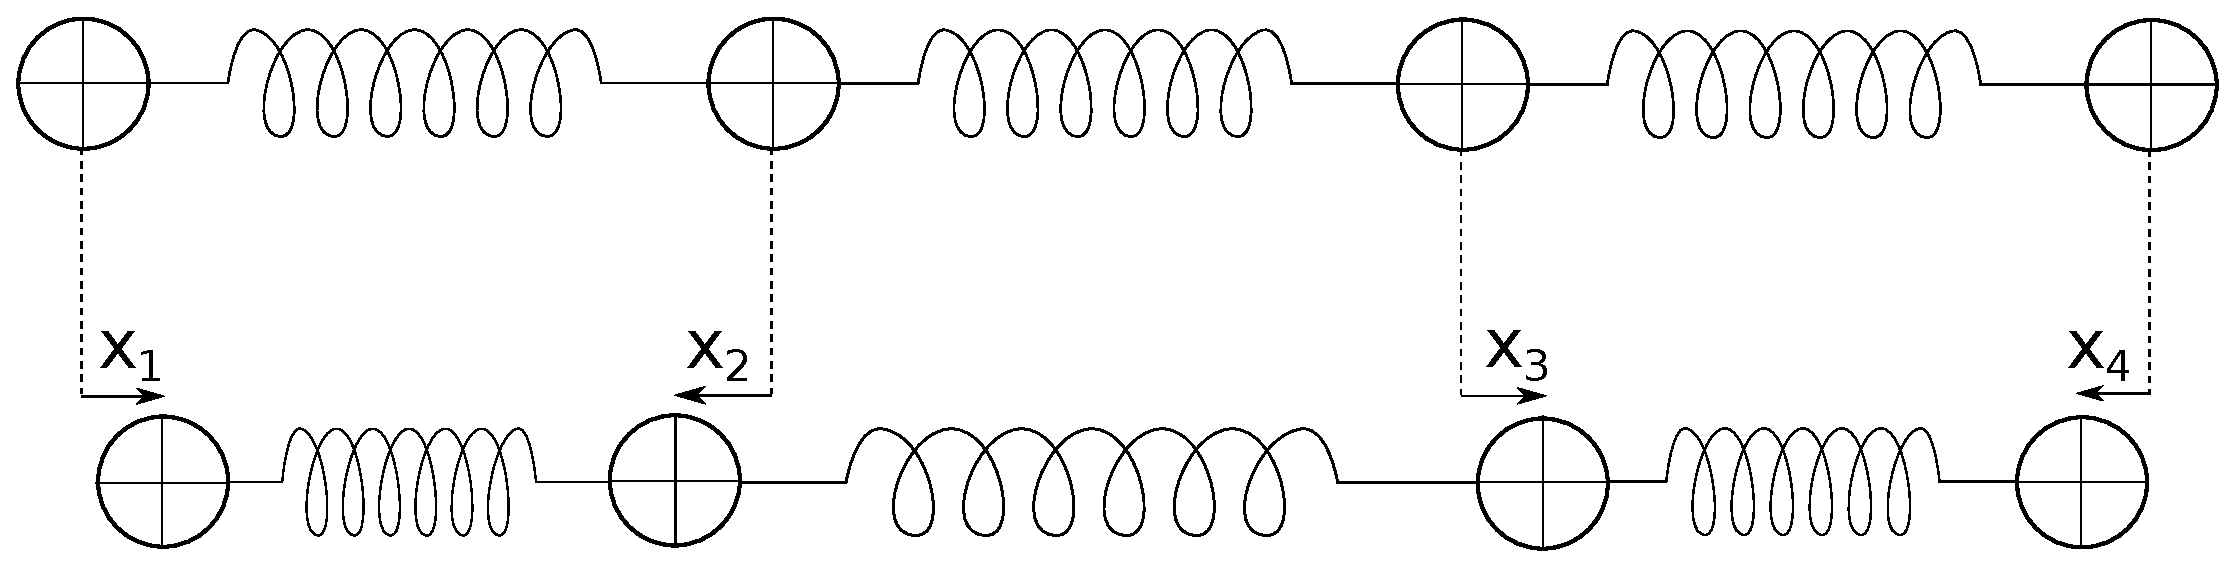
\includegraphics[scale=0.4]{spring4m.eps}
\caption{ressorts couplés}
\label{Res}
\end{figure}


Le principe fondamental de la dynamique appliqué successivement à chaque masse mène à un système
de quatre équations différentielles couplées:

$$
\left \{
\begin{array}{r c l}
m \ddot x_1 &=& -k \, (x_1-x_2)  \\
m \ddot x_2 &=& -k \, (x_2-x_1)  -k \, (x_2-x_3) \\
m \ddot x_3  &=&  -k \,(x_3-x_2) -k \,(x_3-x_4)\\
m \ddot x_4 &=& -k \, (x_4-x_3)  
\end{array}
\right .
\Longleftrightarrow
\left(
\begin{array}{c}
 \ddot x_1 \\  \ddot x_2 \\  \ddot x_3 \\  \ddot x_4
\end{array}
\right) = - {k \over m}
\left(
\begin{array}{rrrr}
1   & -1 & 0  & 0  \\
-1  & 2 & -1 & 0 \\
0  & -1 & 2 & -1 \\
0  & 0 & -1 & 1 \\
\end{array}
\right)
\left(
\begin{array}{c}
x_1 \\ x_2 \\ x_3 \\ x_4
\end{array}
\right)
$$

En se plaçant dans le régime harmonique et en utilisant
la notation complexe, on écrit : $x_i(t)=a_i \, exp(i\omega t)$ où $i \in [1, 4]$ et $a_i \in \mathbbm{C}$.
Noter que les déplacements physiques coïncident avec les parties réelles de ces quantités.\\

On obtient, en notant ${\omega_0^2}=k/m$, le système linéaire suivant:
$$
{\omega_0^2}
\left(
\begin{array}{rrrr}
1   & -1 & 0  & 0  \\
-1  & 2 & -1 & 0 \\
0  & -1 & 2 & -1 \\
0  & 0 & -1 & 1 \\
\end{array}
\right)
\left(
\begin{array}{c}
a_1 \\ a_2 \\ a_3 \\ a_4
\end{array}
\right)=
{\omega^2}
\left(
\begin{array}{c}
a_1 \\ a_2 \\ a_3 \\ a_4
\end{array}
\right) 
$$

Le problème revient à diagonaliser une matrice de couplage que l'on note $K$. 
$$
K=
{\omega_0^2}
\left(
\begin{array}{rrrr}
1   & -1 & 0  & 0  \\
-1  & 2 & -1 & 0 \\
0  & -1 & 2 & -1 \\
0  & 0 & -1 & 1 \\
\end{array}
\right)
$$
où chaque valeur propre  $\lambda$ correspond au carré de la pulsation propre ${\omega}$.

\subsection{Mise en application}

Développer un script Python permettant de déterminer les pulsations propres et les modes associés.
\begin{itemize}
\item La matrice $K$ est une matrice pleine stockée dans un tableau numpy.ndarray.
Les valeurs propres et vecteurs propres sont calculées avec la fonction {\tt linalg.eig} de la librairie {\tt numpy}.
\item La matrice $K$ est une matrice creuse.
On utilisera la fonction {\tt sparse.csr\_matrix} pour stocker les termes non nuls de la
librairie {\tt scipy}.
Les valeurs propres et vecteurs propres sont calculées avec la fonction {\tt sparse.linalg.eigsh} de la librairie {\tt scipy}.
\end{itemize}



\section{Application de conditions de déplacement nul en certains noeuds}

On présente ici une méthode générale pour calculer les modes propres en s'appuyant sur
l'étude précédente lorsque certaines masses du systèmes sont fixes.
Ces conditions s'apparentent aux conditions de dirichlet du type $x_i=0$.

En notant $N_d$ le nombre de masses où  la condition de dirichlet est imposée, 
le nombre de degrés de liberté se réduit alors à $N_{dof}=N-N_d$ et correspond 
ici au nombre de masses pouvant osciller.\\

\subsection{Algorithme}
L'algorithme consiste à former une liste $l$ où le numéro de chaque masse pouvant osciller,
apparaît de façon unique. Sa
taille est $N_{dof}=N-N_d$ et s'identifie, ici,  au nombre de degrés de liberté. \\

On forme ensuite une matrice de projection $P$ permettant de passer de l'espace des solutions à $N$ degrés de 
liberté (étude précédente) à celui restreint à $N_{dof}$ degrés de liberté.
Les dimensions de P sont $N_{dof} \times N$ (nombre de lignes $\times$ nombre de colonnes).
On initialise d'abord la matrice $P$ à zéro;
puis en parcourant séquentiellement la liste $l$, on impose $P[i, l[i]]=1$ avec $i \in [1, N_{dof}]$.
On remarque que $P P^t = {\tt Id}(N_{dof})$ .\\

Une autre façon de construire la matrice $P$ est de l'initialiser avec  la matrice identité ${\tt Id}(N)$
puis de supprimer toutes les lignes correspondant aux noeuds de dirichlet. Cette technique
est bien adaptée à Numpy/Scipy en masquant les numéros de lignes correspondant aux noeuds de dirichlet.


\begin{lstlisting}[language=Python]
def delete_rows(mat, indices):
    indices = list(indices) # transformation en liste
    mask = np.ones(mat.shape[0], dtype=bool) # ligne de True
    mask[indices] = False # True->False pour les noeuds de dirichlet
    return mat[mask]
\end{lstlisting}

\begin{figure}[!h]
\centering
\includegraphics[scale=0.25]{matP.eps}
\caption{exemple de matrice $P$ avec $ld=[0, 2]$}
\label{matP}
\end{figure}

On construit ensuite $K_p$ qui est la matrice projetée de $K$ dans l'espace
solution à $N_ {dof}$ degrés de liberté: $K_p=P K P^t$ .
C'est cette matrice qui est finalement diagonalisée. On obtient alors les valeurs propres $\lambda_p$ associées
aux vecteurs propres $a_p$. Autrement dit, cela revient à résoudre:
$P K P^t a_p= \lambda_p a_p$.

On reconstruit la solution dans l'espace à $N$ corps en appliquant $a=P^t a_p$. 
Elle vérifie automatiquement, $a[i]=0$ pour tout noeud $i$ de dirichlet.

\subsection{Mise en application}

$\bullet$ Utiliser sous Numpy, la fonction {\tt ld=numpy.unique(ld)} pour éliminer tout doublon dans la liste {\tt ld}.

$\bullet$ Calculer numériquement les modes propres du système lorsque les masses $0$ et $2$ sont fixes.

$\bullet$ Vérifier vos résultats numériques avec une approche analytique.

\end{document}